\section*{Fra Pilestredet til Teknisk museeum}

Destinasjonen vår er er gitt ved en gateadresse, Kjelsåsveien $k$, og oppgaven vår er dermed å finne ut hva $k$ er. Vi har gitt at $k=p\cdot q$, hvor $(p,q)$  danner et tvillingprimtallspar, så la oss først liste opp noen av disse. Tvilling primtall er primtall som er kun $2$ heltall fra hverandre, altså at både $p$ og $p+2$ er primtall. Et eksempel er $3$ og $5$, som også er det første tvillingprimtallsparet. Merk at $2$ og $3$ ikke regnes som et tvillingprimtall. De første fem parene er $(3,5)$, $(5,7)$, $(11,13)$, $(17,19)$ og $(29,31)$. 

Den neste biten med informasjon vi får oppgitt er at $(p,q)$ er det $n$’te tvillingprimtallsparet. Så la oss nå prøve å finne ut hva $n$ kan være. Tallet $n$ skal være antall Platonske legemer i dimensjon $k$, noe som gjør at vi har et slags rekursivt definert problem. Men først, hva er en Platonsk legeme? Matematisk presist er det et konvekst legeme bestående av regulære like polyhedre, men dette kan mye bedre forklares ved å vise et eksempel: 

\begin{center}
    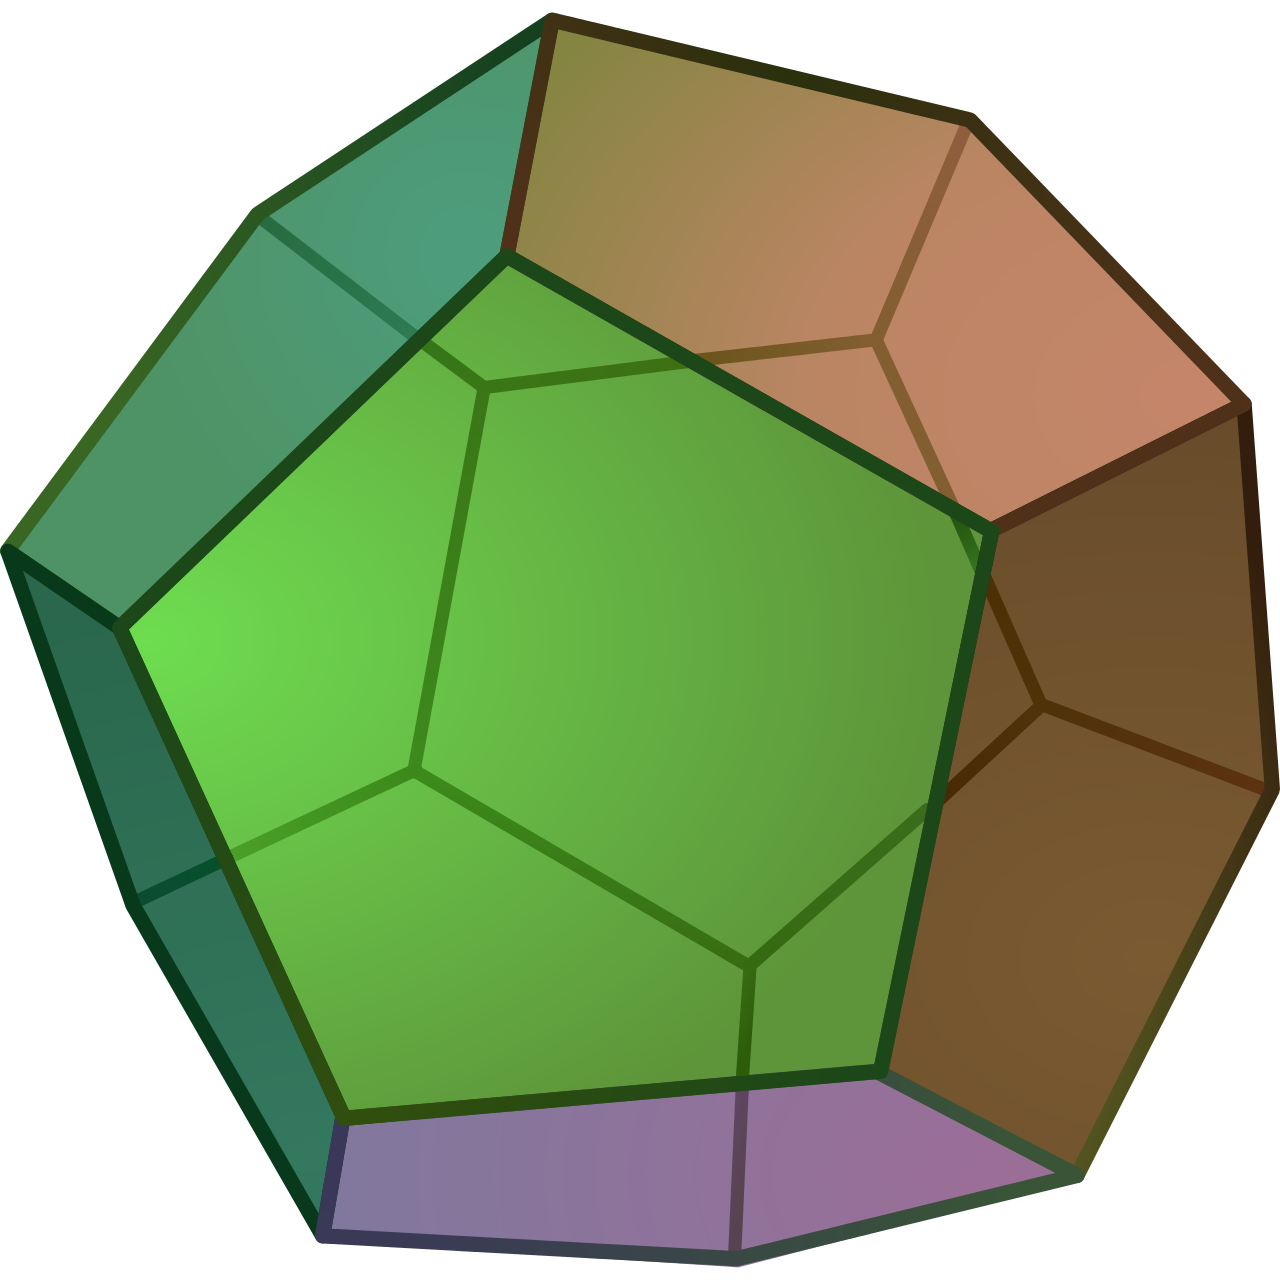
\includegraphics[height = 7cm]{img/Dodecahedron.png}    
\end{center}

Her ser vi at legemet består av av $12$ helt like femkanter, og at ingenting rart stikker ut noen sted. Dette er altså et Euklidsk legeme i dimensjon $3$. I dimension tre har vi fem slike legemer, som kalles for tetraederet,

\begin{center}
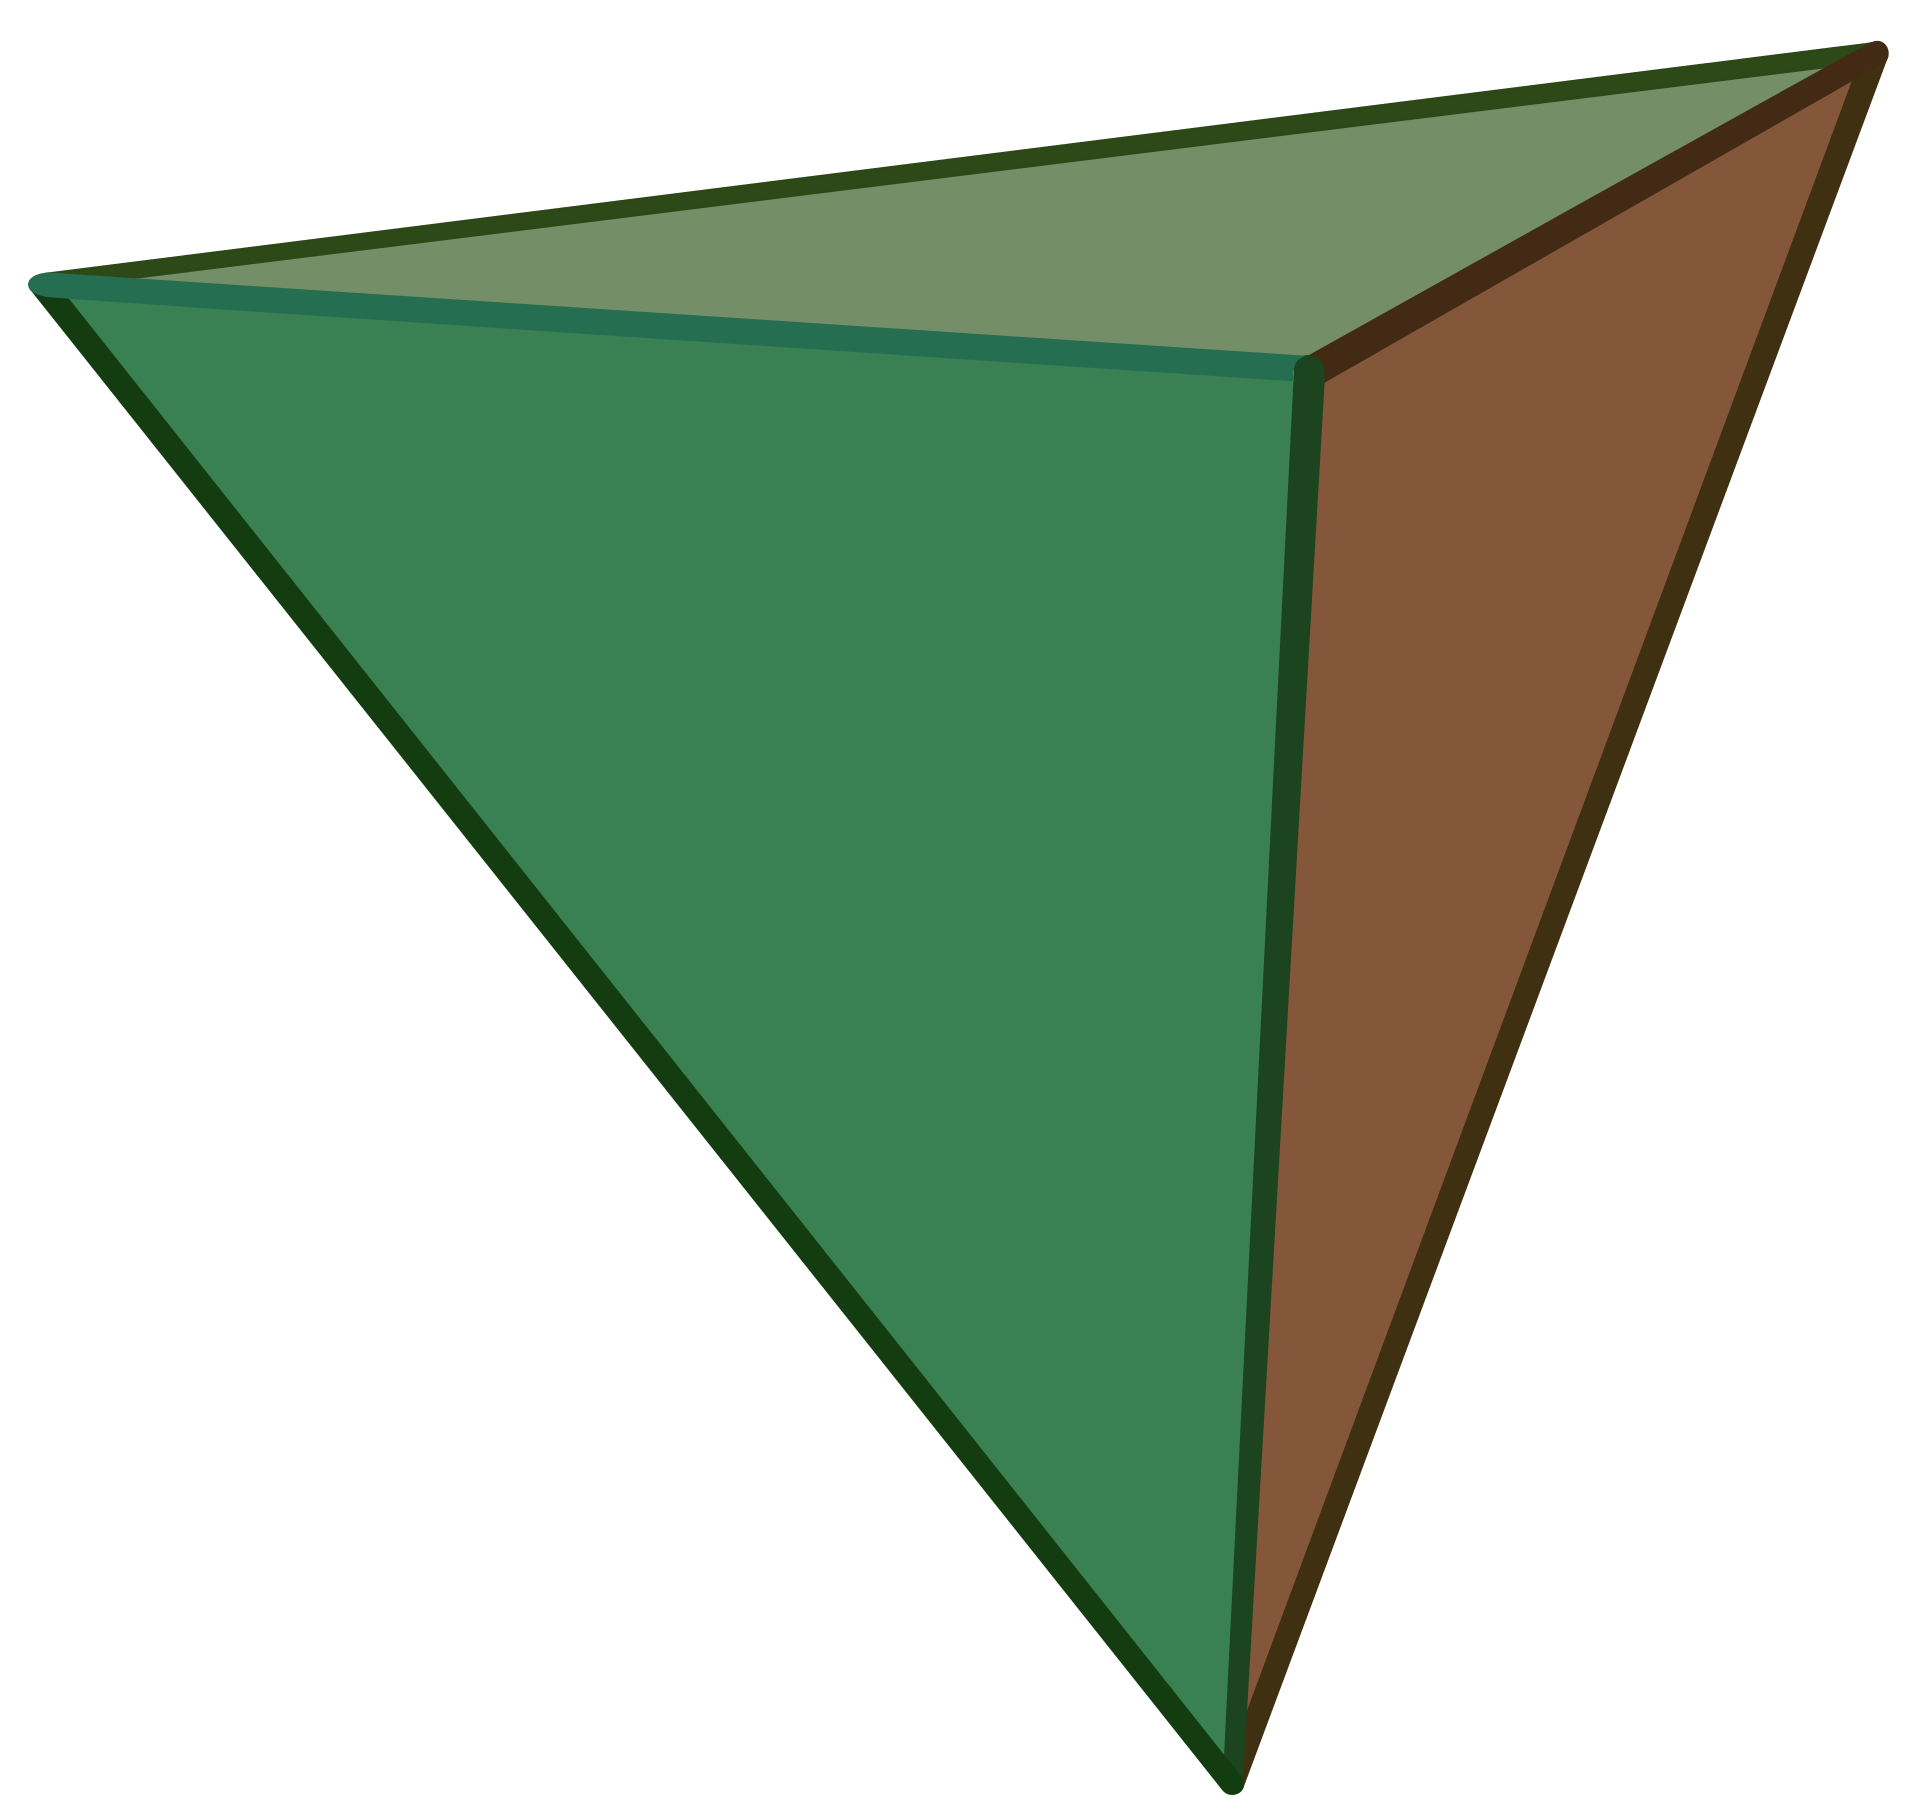
\includegraphics[height = 6cm]{img/Tetrahedron.png}
\end{center}

heksaederet, bedre kjent som en kube,

\begin{center}
    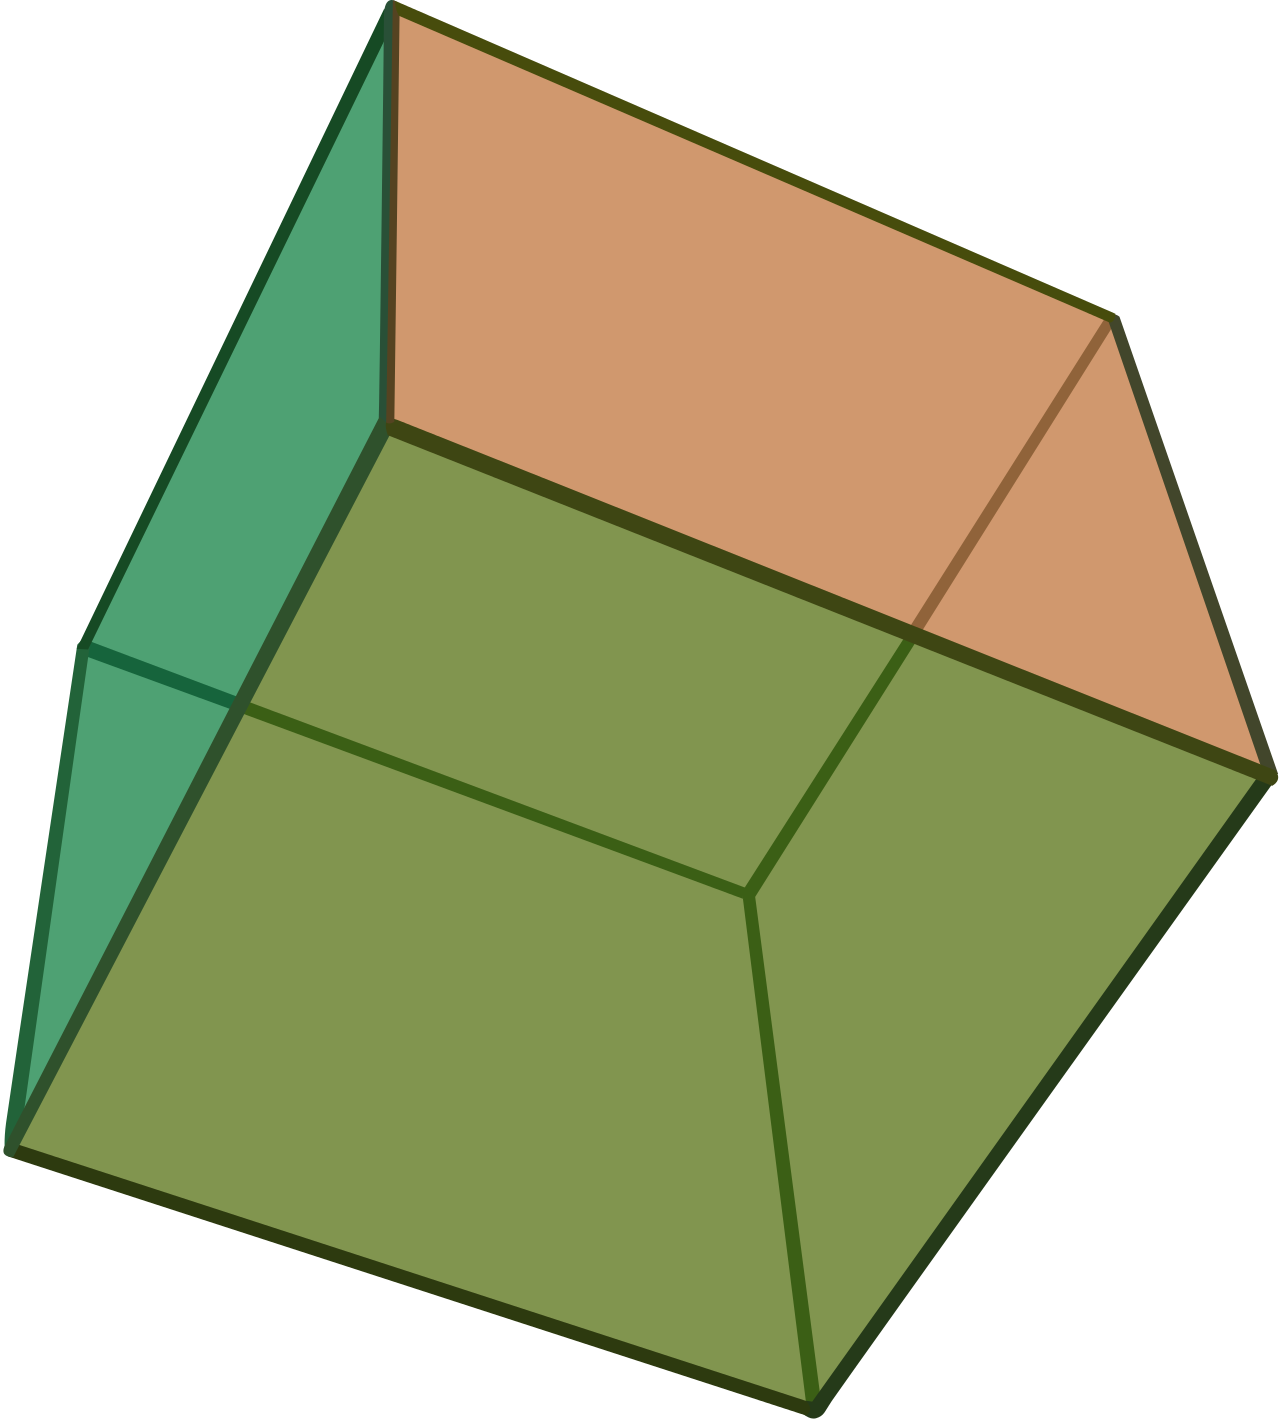
\includegraphics[height = 6cm]{img/Hexahedron.png}
\end{center}

oktaederet,

\begin{center}
    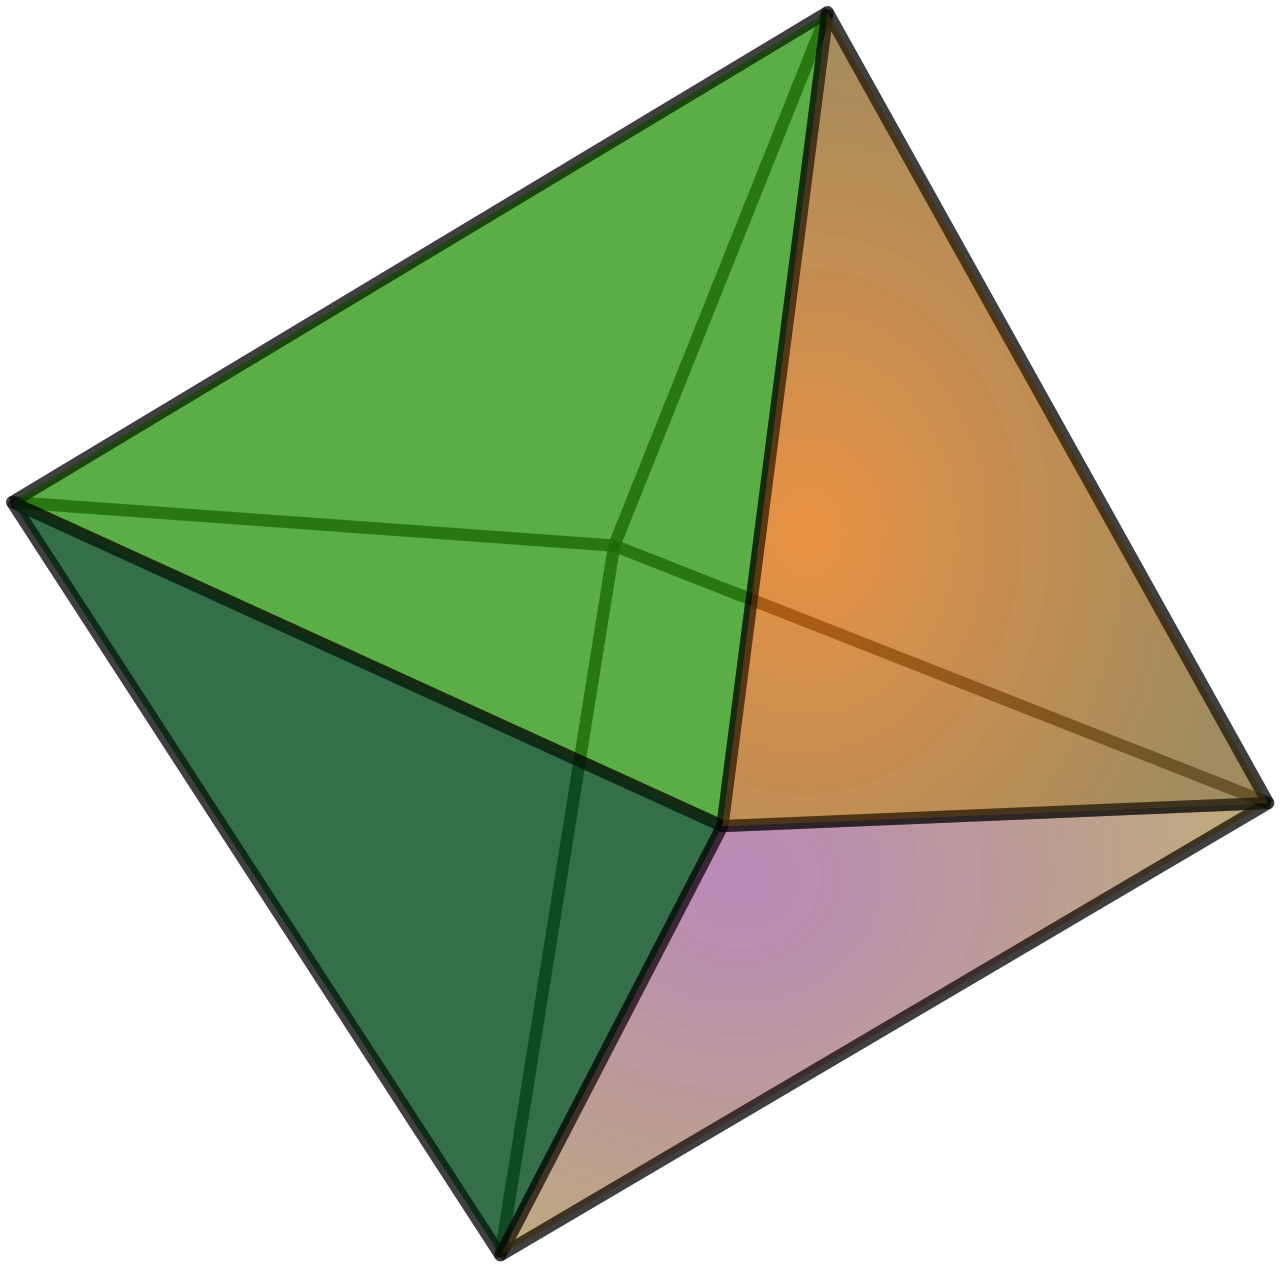
\includegraphics[height = 6cm]{img/Octahedron.png}
\end{center}

dodekaederet,

\begin{center}
    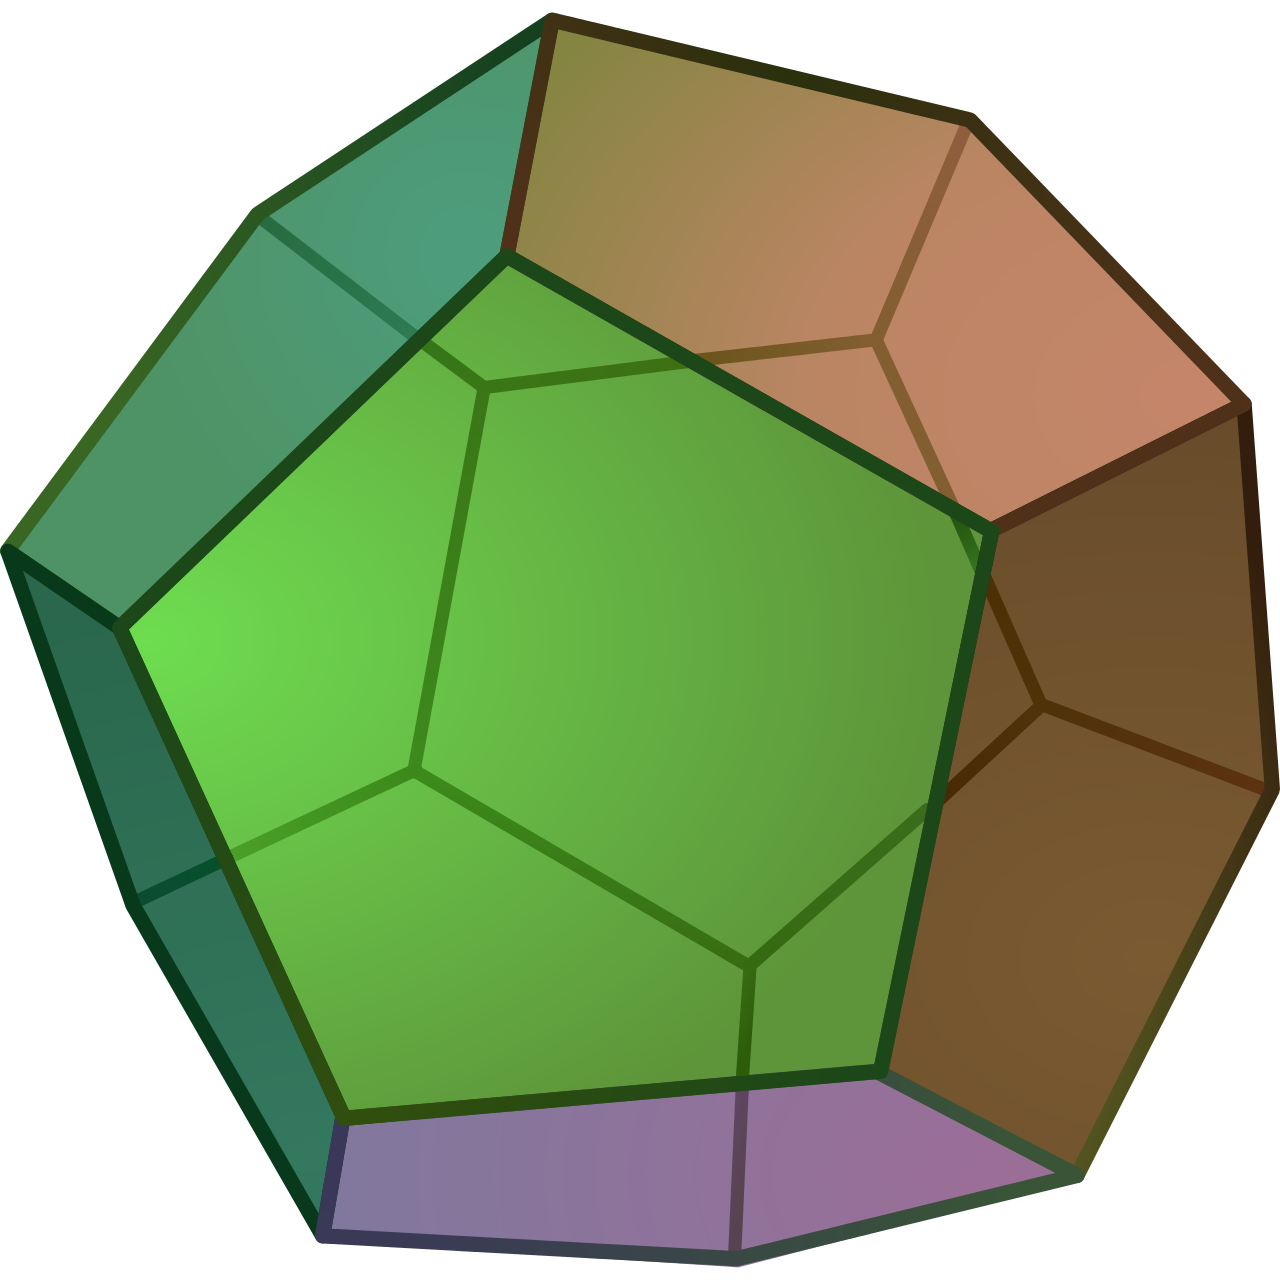
\includegraphics[height = 6cm]{img/Dodecahedron.png}
\end{center}

og til slutt ikosaederet, 

\begin{center}
    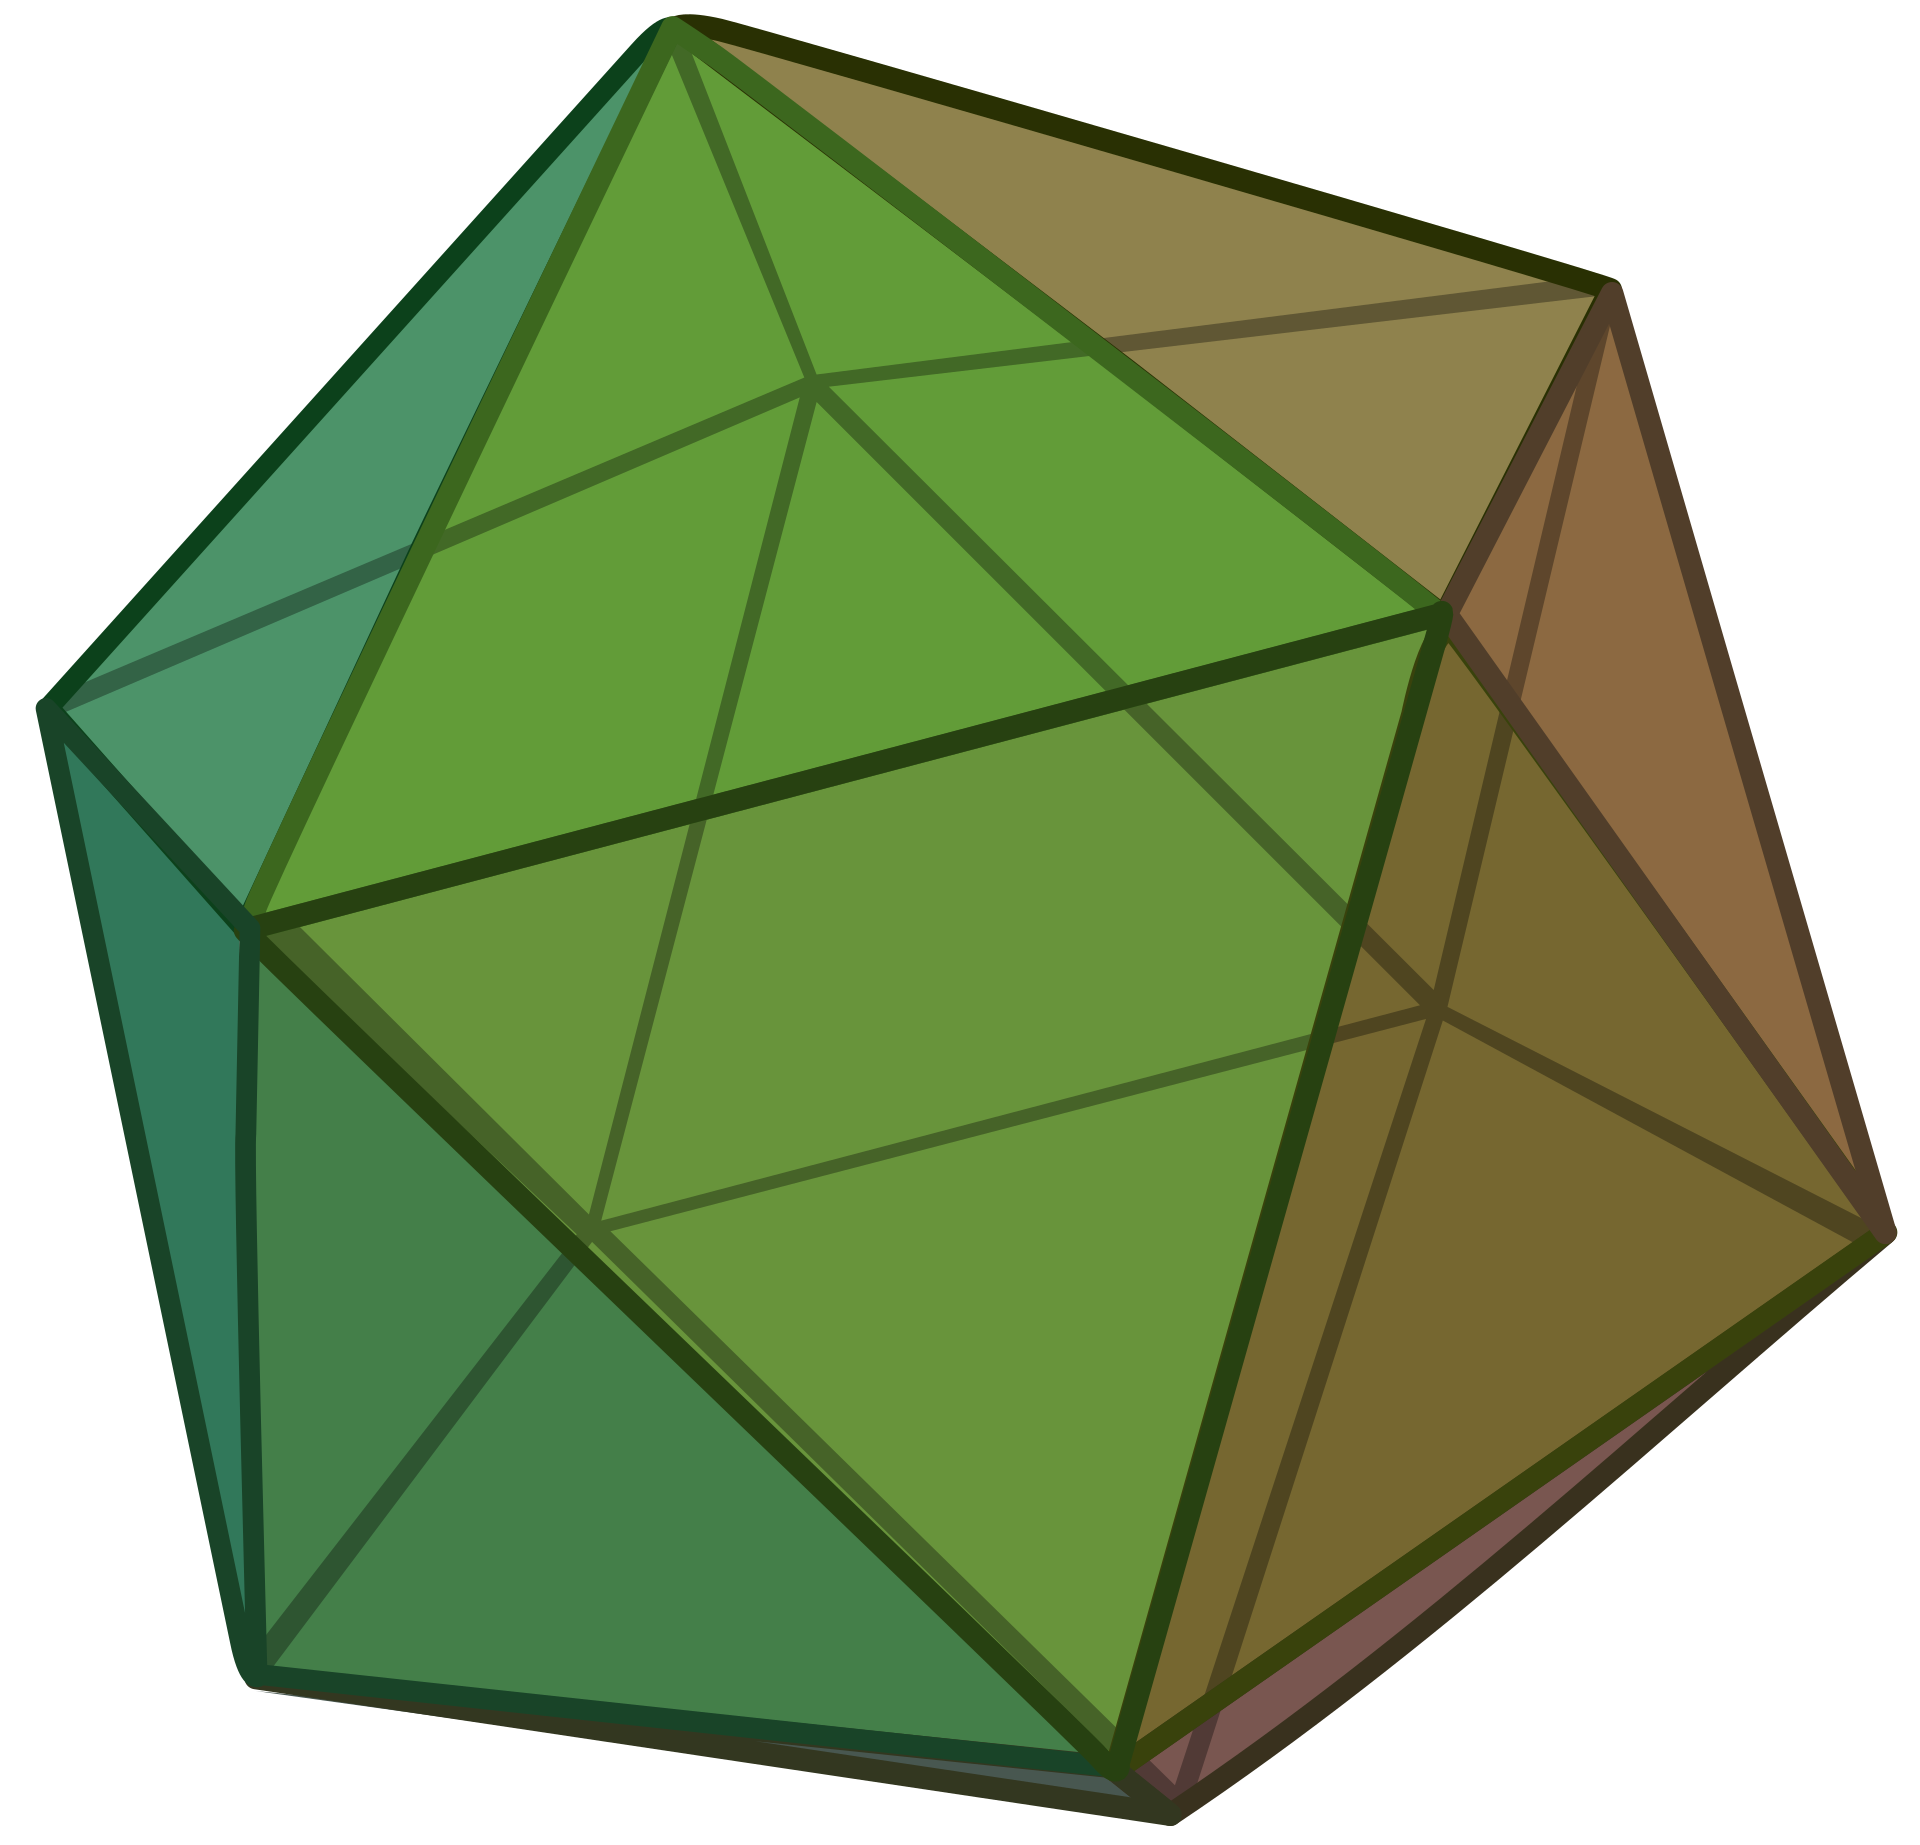
\includegraphics[height = 6cm]{img/Icosahedron.png}
\end{center}

De første tre kan vi beskrive som en trekantet pyramide, en kube og to sammensatte pyramider. Husk disse, de er viktige senere. 

Vi kan lage tilsvarende legemer i alle mulige dimensjoner, ved å sette samme de høyere dimensjonale analogene til polygoner, altså polyhedre. I dimensjon $2$ er det kun linjestykker vi kan sette sammen, så dermed er alle polygoner faktisk Platonske legemer. Vi kan lage polygoner med et vilkårlig antall sidestykker, så det er dermed uendelig antall Platonske legemer i dimensjon $2$. I dimensjon $1$ har vi kun et punkt å bygge disse legemene fra, noe som ikke gir oss mye spillerom. Det er bare et måte å sette sammen et punkt på, som vil si at vi kun har ett Platonsk legeme i dimensjon $1$. 

Det spennende skjer når vi øker dimensjonen over $3$. I dimensjon $4$ har vi litt ekstra rom til å sette sammen figurer, og det er faktisk akkuratt nok rom til å sette sammen et ekstra legeme, så vi har faktisk seks Platonske legemer i dimensjon $4$. Man skulle kanskje tro at dette fenomenet fortsatte i høyere dimensjoner, at man alltid fikk litt mer og mer plass til å lage nye legemer, men dette er faktisk ikke tilfellet. I høyere dimensjoner tar også byggestenene — polyhederene — mer og mer plass, og etter dimensjon $4$ kansellerer disse to effektene hverandre. I alle dimensjoner høyere enn $4$ er det faktisk bare plass til å lage $3$ Platonske legemer! Vi kan alltid lage en høyere dimensjonal kube, en høyere dimensjonal trekantet pyramide, og en høyere dimensjonal versjon av to sammensatte pyramider. 

Så, hvis vi lager en liste med hvor mange Platonske legemer det er i alle dimensjonene får vi 

$$
1,\infty, 5, 6, 3, 3, 3, 3,\ldots
$$

Vi har nå all informasjonen vi trenger til å løse oppgaven. Vi vet at $k=p\cdot q$ der $(p,q)$ er et primtallspar. Vi tester med det første primtallsparet, altså $n=1$, som gir $p=3, q=5$. Da er $k = 15$, men her har vi at $n=1$ ikke er antall Platonske legemer i dimensjon $15$, så dette kan ikke være riktig primtallspar. Vi ser at alle primtallspar vil gi et tall $k$ som er større enn $4$, altså vil alltid antall Platonske legemer i dimensjon $k$ være $3$, uansett hvilket primtallspar vi velger. Dette betyr at $n$ må være lik $3$, som igjen gir at $(p,q) = (11,13)$ ettersom $(11,13)$ er det tredje primtallsparet. Dette gir $k=11\cdot 13 = 143$. Dette tallet gir en gyldig løsning ettersom

\begin{itemize}
    \item $(11,13)$ er et primtallspar
    \item $(11,13)$ er det tredje primtallsparet, altså $n=3$
    \item $n=3$ er antall Platonske legemer i dimensjon $k=11\cdot 13 = 143$
\end{itemize}

Denne løsningen er også unik ettersom alle andre primtallspar vil gi en feil verdi for $n$. Dermed er destinasjonen vår Kjelsåsveien 143, som er adressen til Teknisk museum!